\section{Bedienung des Rastertunnelmikroskops}\label{sec:versuch}
Bei der Versuchsdurchführung wird ein RTM mit einem externen Controller und der zugehörigen Software \texttt{Easyscan 2} verwendet.
Der Experimentierplatz ist in \cref{fig:versuchsplatz} gezeigt.
\begin{figure}[H]
	\centering
	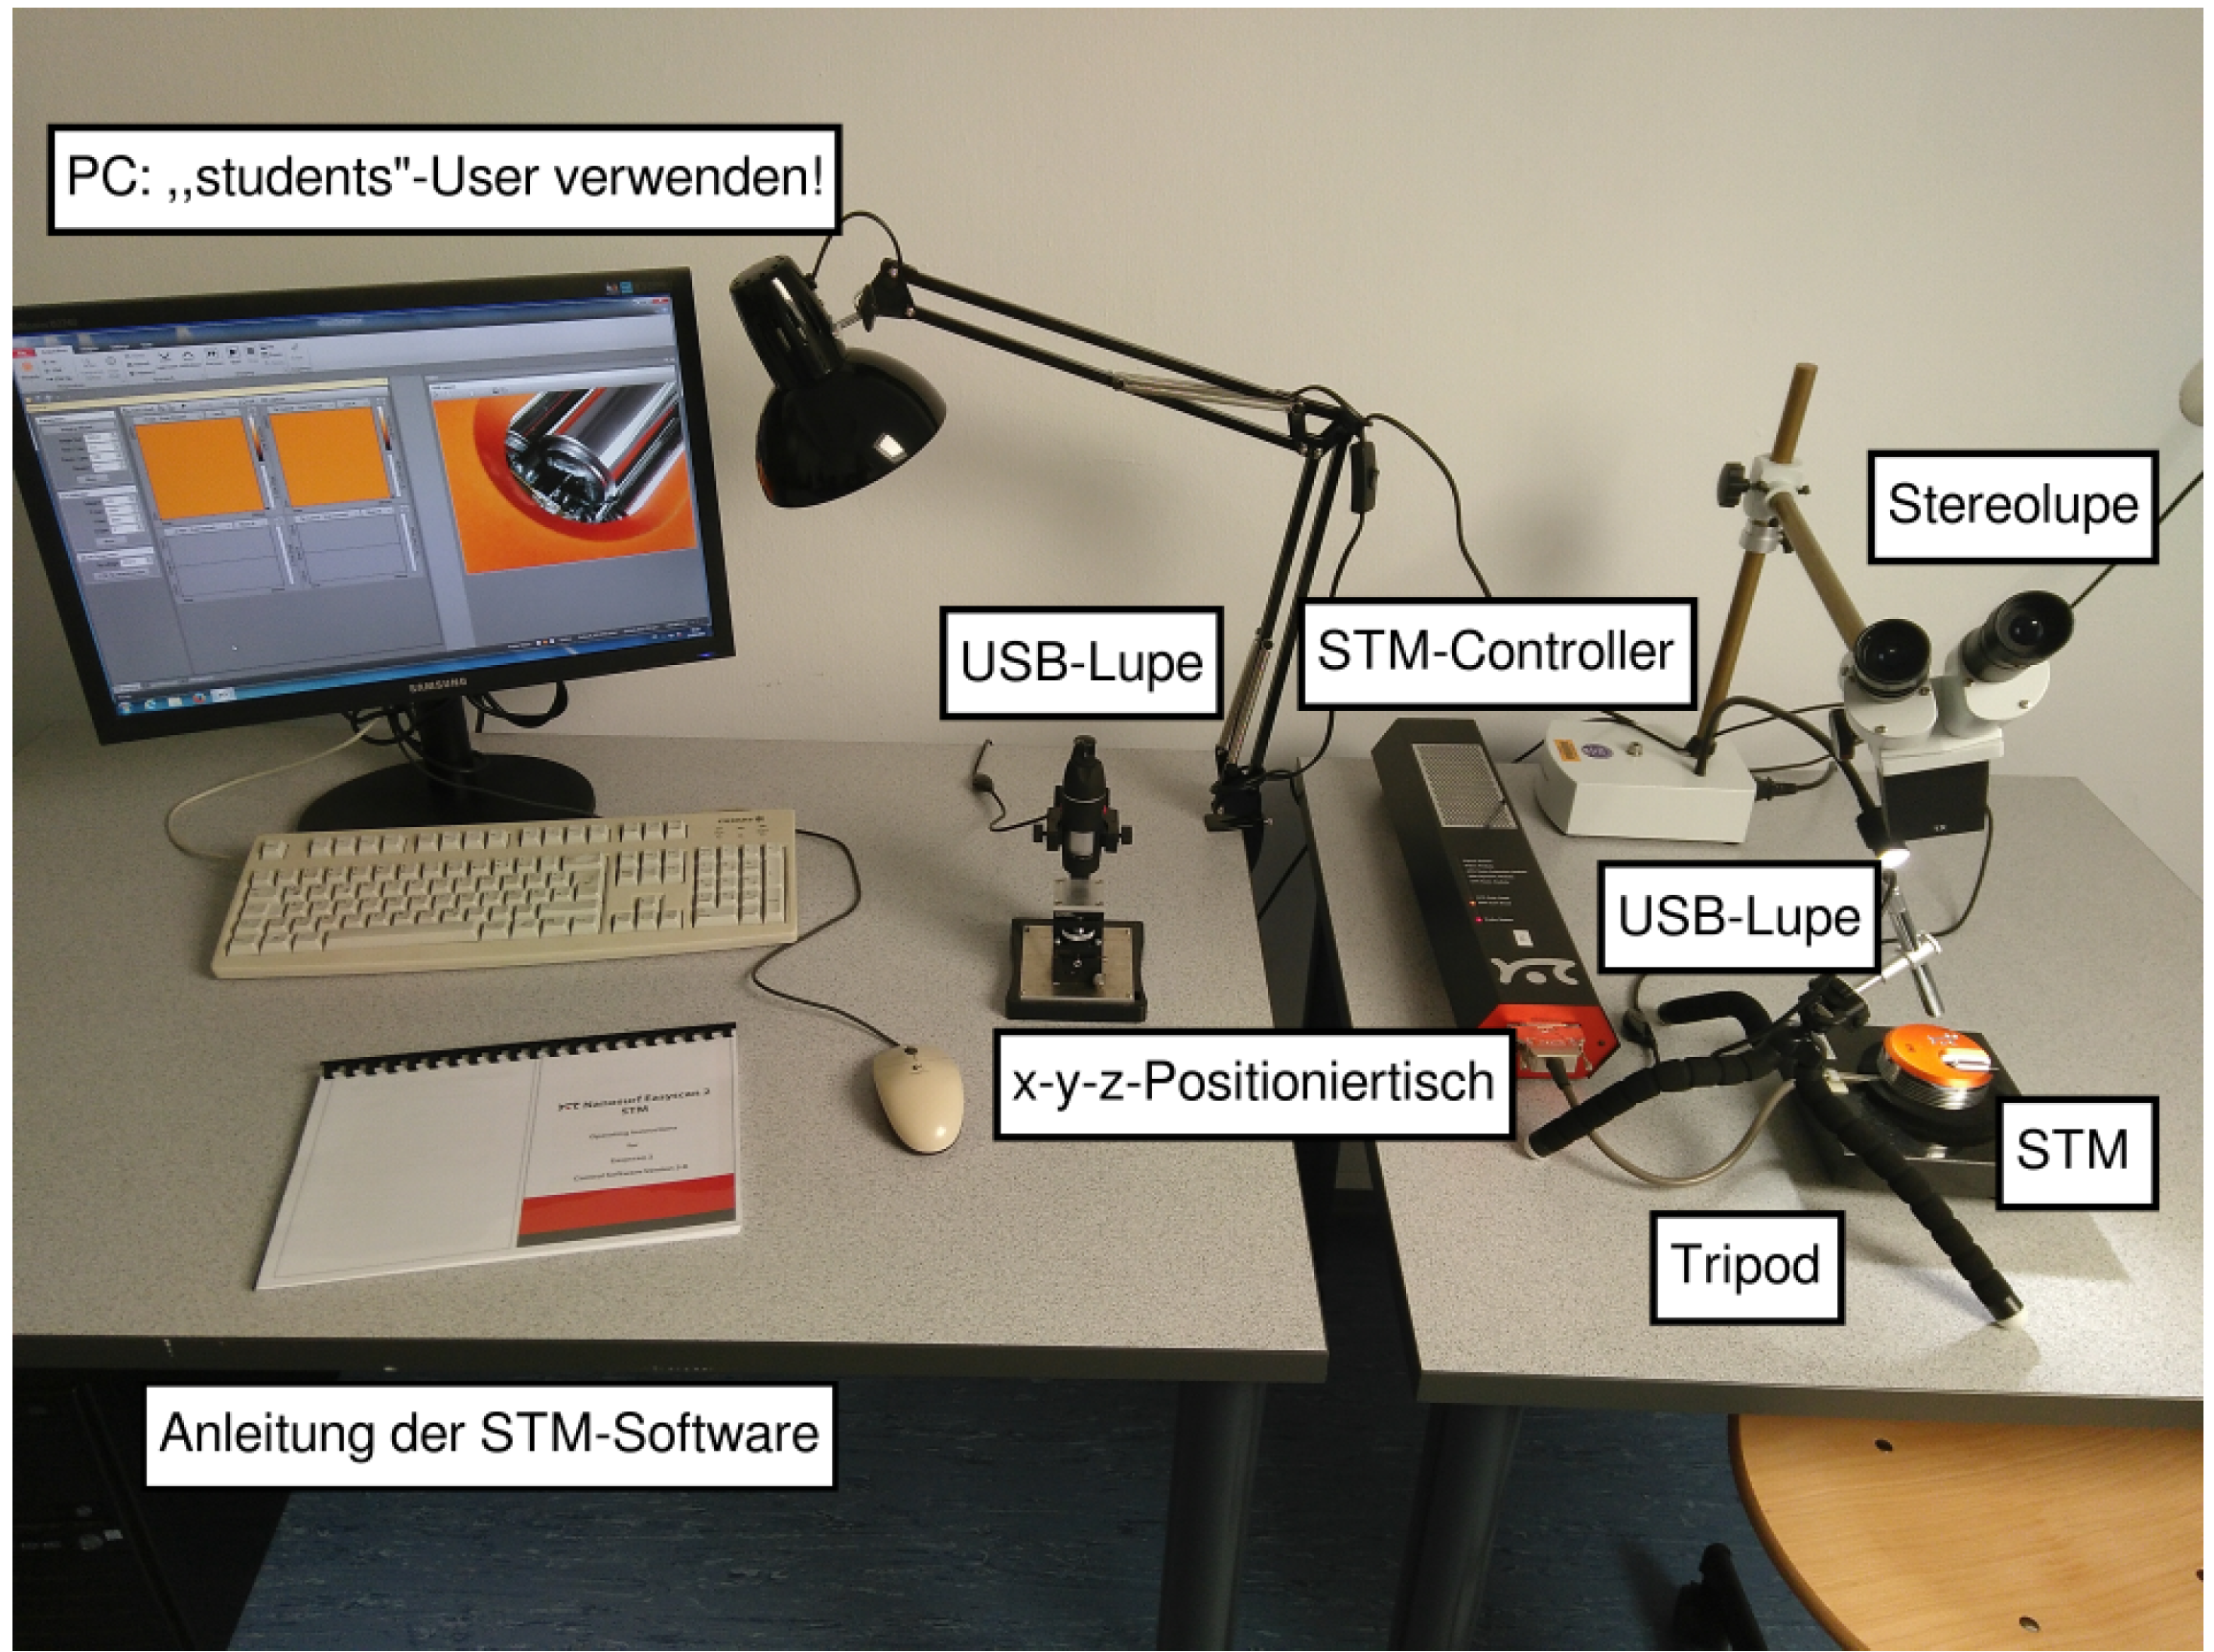
\includegraphics[width=0.8\linewidth]{../figs/versuchsplatz.png}
	\caption{Experimentierplatz mit RTM und dem notwendigen Zubehör (Quelle: \cite{skript})}
	\label{fig:versuchsplatz}
\end{figure}
Um mit dem RTM arbeiten zu können, wird der RTM-Controller über einen Kippschalter eingeschaltet. Anschließend wird der beistehende Rechner
hochgefahren, um die für den RTM-Controller benötigte Software \texttt{Easyscan 2} zu öffnen. Außerdem ist der Arbeitsbereich mit den Eingabegeräten
des Rechners (Tastatur und Maus) auf einem anderen Tisch als das RTM platziert, sodass die vielen Berührungspunkte der Hände, Arme, Füße und Beine mit dem Tisch während der Bedienung
der Software keinen Einfluss auf die Arbeitsweise des RTMs haben. Ohnehin ist das RTM auf einem schwingungsdämpfenden Körper befestigt, um
den Einfluss von Vibrationen auf die Messungen zu verringern, allerdings hat sich bei der Versuchsdurchführung tatsächlich gezeigt, dass leichte Zusammenstöße
mit dem RTM-Tisch zu kurzzeitigen Ausreißern während eines Messprozesses führen, weshalb eine Aufteilung der beteiligten Arbeitsgeräte definitv sinnvoll ist.\par
Auf dem Tisch mit dem Rechner ist zudem eine USB-Lupe positioniert, mit der die verwendeten Proben und Spitzen auf ihre Qualität untersucht werden können.
Für diese USB-Lupe wird eine separate Software verwendet.\par
Das RTM weißt eine Öffnung auf, in welche die Spitze und Probe eingesetzt werden können. Diese Öffnung ist mit einer Schutzkappe abgedeckt, welche aber für
die Versuchsdurchführung entfernt werden kann. Darüber hinaus wird eine weitere USB-Lupe (montiert auf einem Dreibein) auf die Öffnung des RTMs gerichtet,
um später die Annäherung der Probe an die Spitze beobachten zu können. Das resultierende Bild dieser USB-Lupe kann in \texttt{Easyscan 2} dargestellt werden.\par
Die Proben, der Spitzendraht und das benötigte Zubehör befindet sich in einer Box (siehe \cref{fig:koffer}).
\begin{figure}[H]
	\centering
	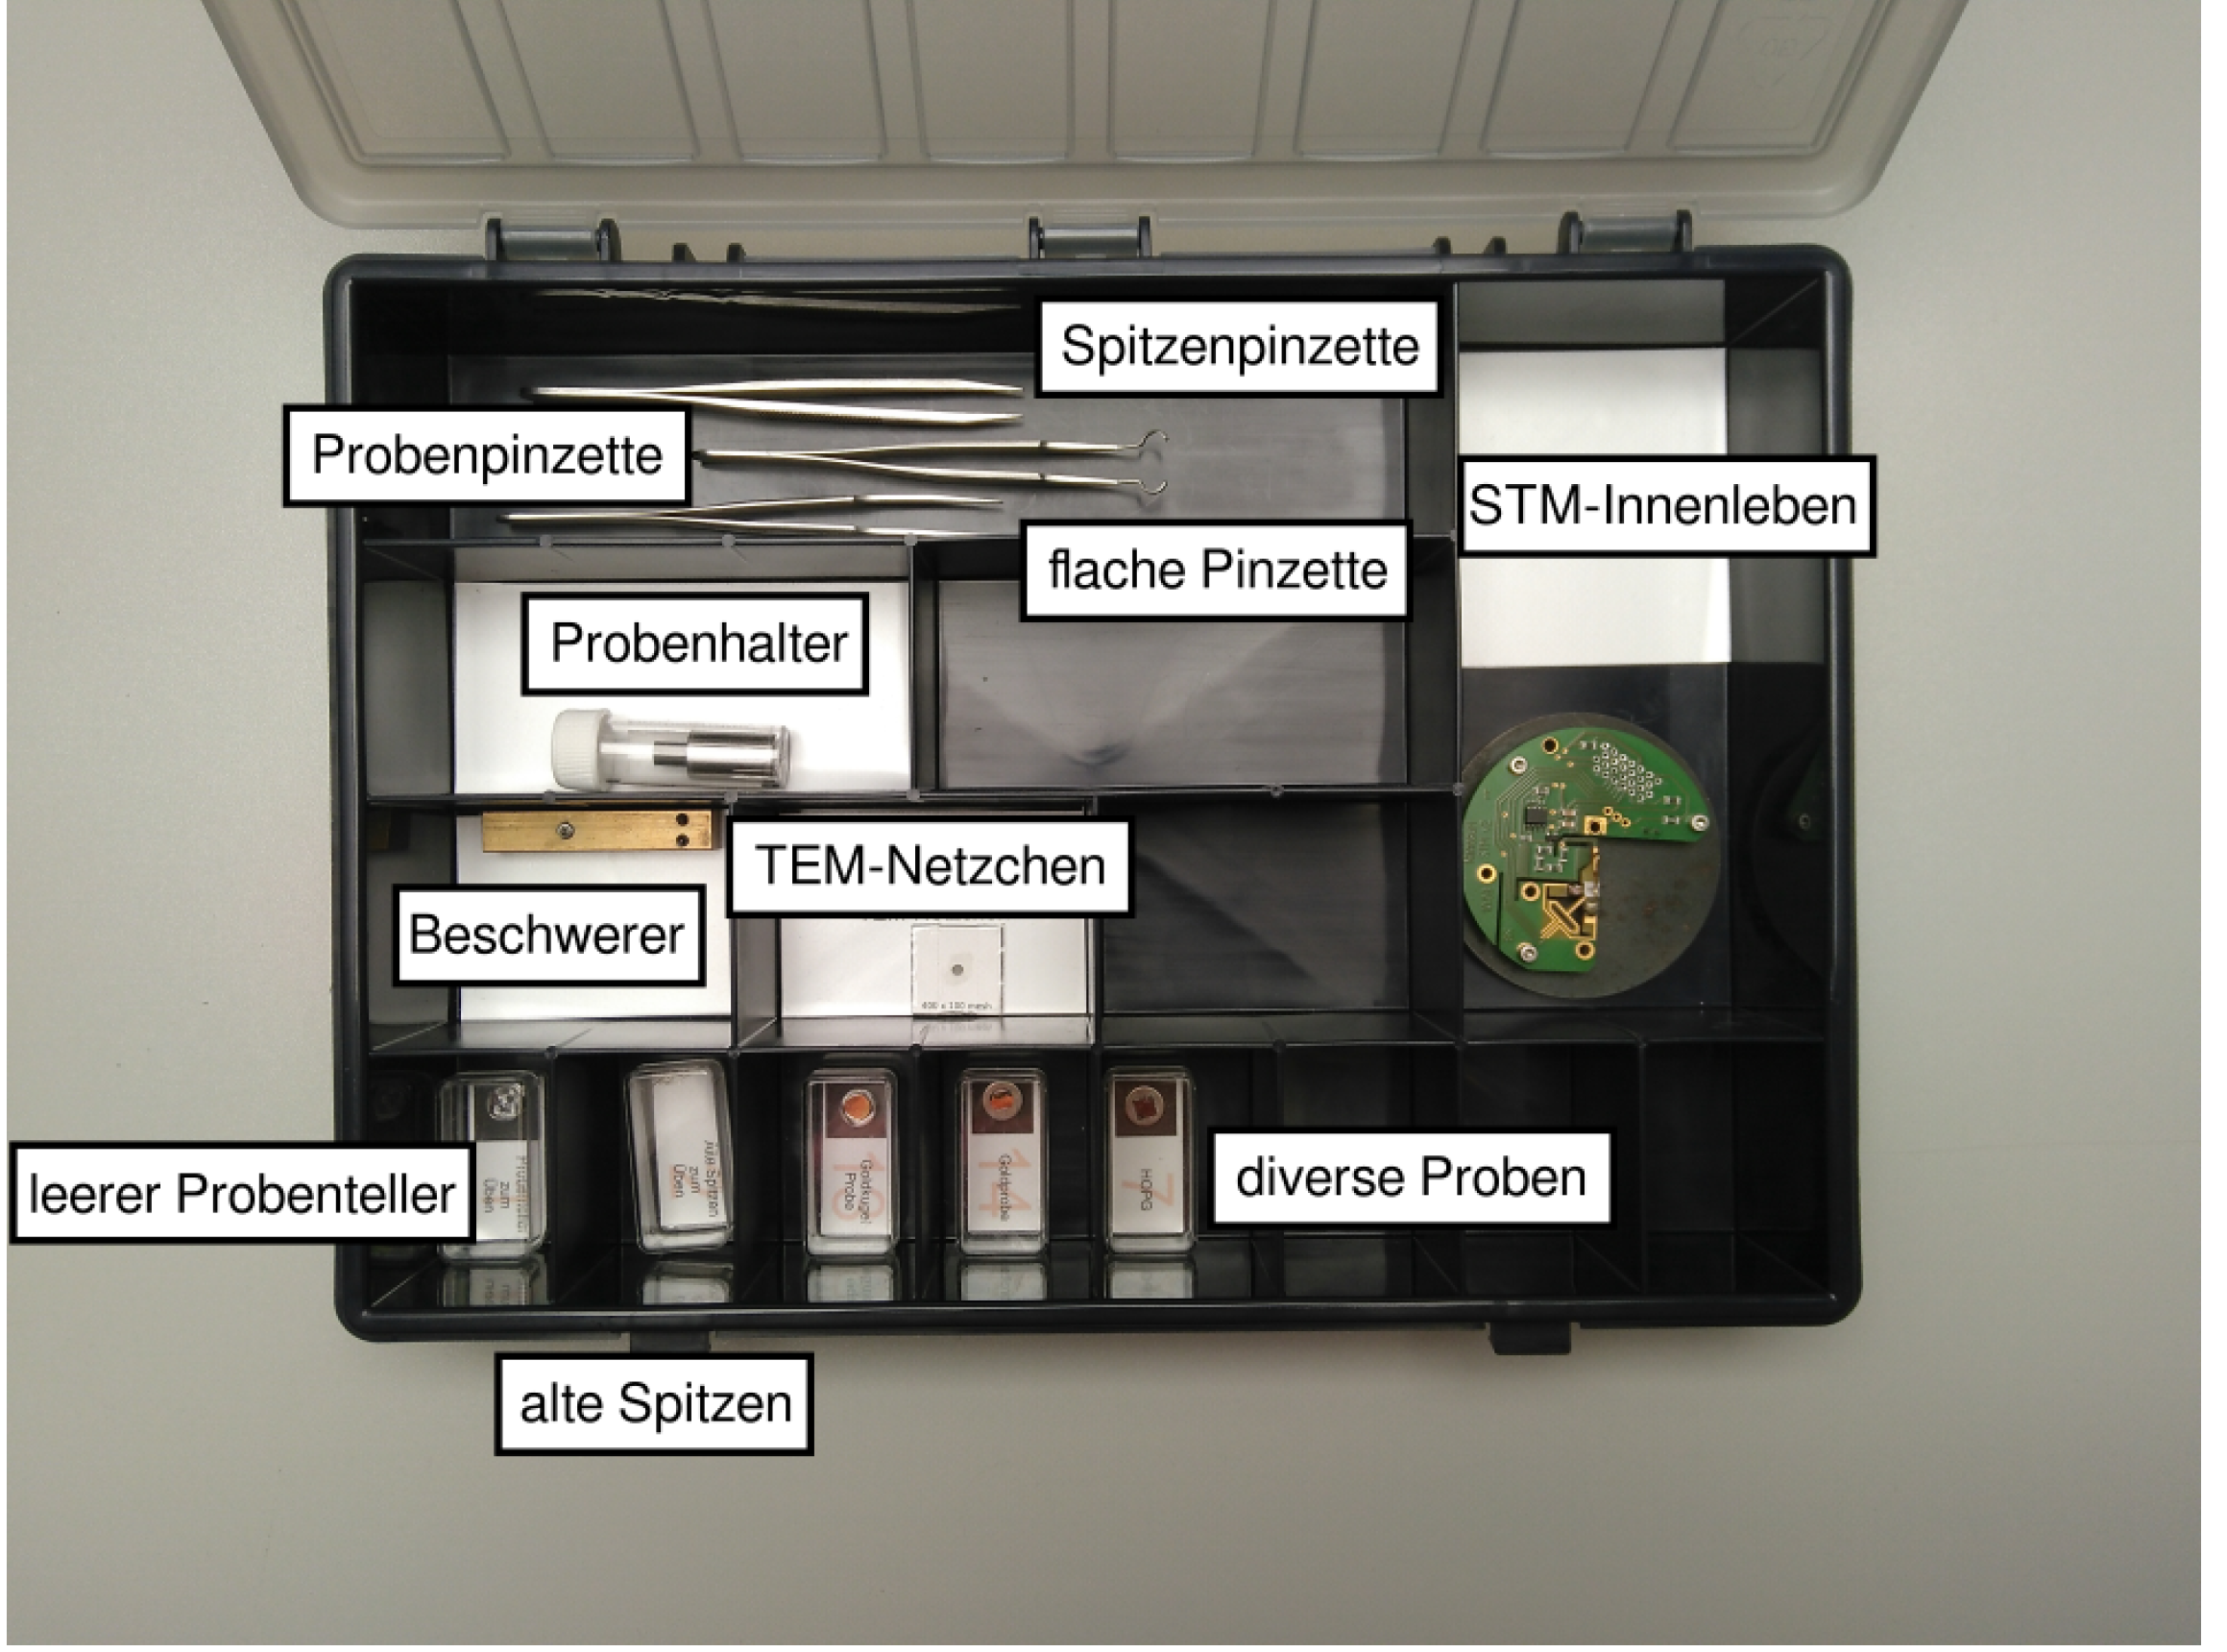
\includegraphics[width=0.8\linewidth]{../figs/koffer.png}
	\caption{Box mit den Proben und dem benötigten Zubehör (Quelle: \cite{skript})}
	\label{fig:koffer}
\end{figure}